\documentclass[12pt,border=2mm]{standalone}
\usepackage{pgfplots}
\usepgfplotslibrary{groupplots,fillbetween}
\pgfplotsset{compat=1.18}
\definecolor{BCred}{rgb}{0.7, 0.11, 0.11}
\definecolor{BCblue}{rgb}{0.0, 0.20, 0.42}
\definecolor{BCgreen}{rgb}{0.11, 0.35, 0.02}
\pgfplotsset{every axis/.append style={width=7.5cm, height=7.5cm, scale only axis,
  ticklabel style={font=\small, /pgf/number format/fixed},
  yticklabel style={text width=10mm, align=right},
  label style={font=\normalsize}, title style={font=\normalsize},
  legend style={draw=none, font=\small}}}
\begin{document}
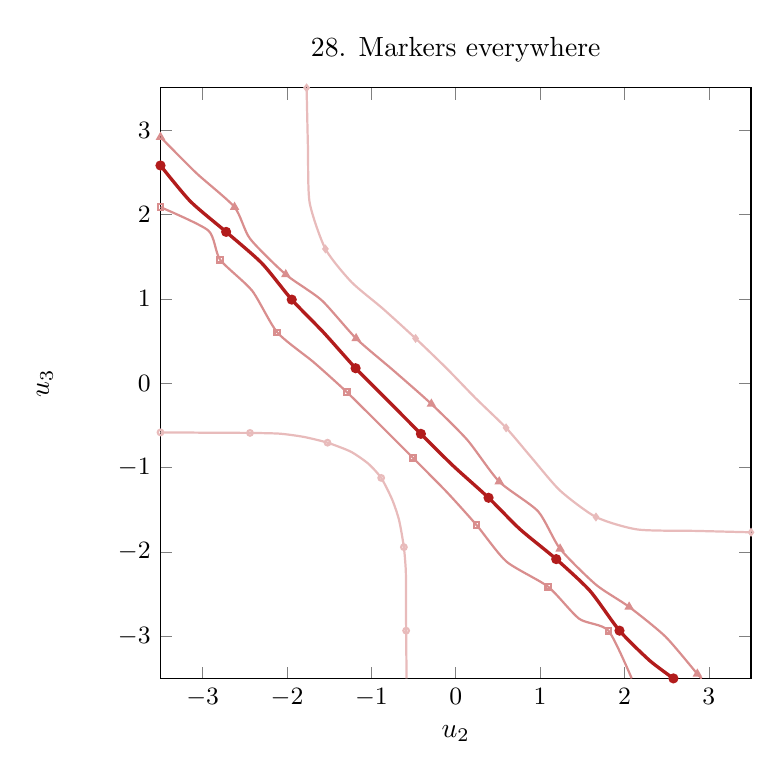
\begin{tikzpicture}
\begin{groupplot}[group style={group size=1 by 1}]
\nextgroupplot[xmin=-3.5, xmax=3.5, ymin=-3.5, ymax=3.5, xlabel={$u_2$}, ylabel={$u_3$}, axis equal image, title={28. Markers everywhere}]
\addplot[thick,color=BCred!30,smooth,tension=0.4,mark=o,mark size=1pt,mark repeat=3] coordinates {(-3.500,-0.584)(-3.146,-0.586)(-2.793,-0.589)(-2.439,-0.590)(-2.086,-0.599)(-1.803,-0.637)(-1.520,-0.706)(-1.243,-0.813)(-1.036,-0.955)(-0.884,-1.123)(-0.754,-1.379)(-0.672,-1.623)(-0.615,-1.944)(-0.592,-2.227)(-0.590,-2.581)(-0.588,-2.934)(-0.585,-3.288)(-0.584,-3.500)};
\addplot[thick,color=BCred!50,smooth,tension=0.4,mark=square,mark size=1pt,mark repeat=2] coordinates {(-3.500,2.086)(-2.934,1.810)(-2.793,1.463)(-2.414,1.096)(-2.115,0.601)(-1.683,0.247)(-1.291,-0.106)(-0.884,-0.509)(-0.509,-0.884)(-0.106,-1.291)(0.247,-1.683)(0.601,-2.115)(1.096,-2.414)(1.463,-2.793)(1.810,-2.934)(2.086,-3.500)};
\addplot[very thick,color=BCred,smooth,tension=0.4,mark=*,mark size=1.2pt,mark repeat=2] coordinates {(-3.500,2.580)(-3.146,2.155)(-2.722,1.793)(-2.298,1.421)(-1.944,0.990)(-1.567,0.601)(-1.187,0.177)(-0.813,-0.199)(-0.413,-0.601)(-0.035,-0.976)(0.389,-1.359)(0.762,-1.732)(1.191,-2.086)(1.591,-2.462)(1.941,-2.934)(2.298,-3.288)(2.580,-3.500)};
\addplot[thick,color=BCred!50,smooth,tension=0.4,mark=triangle,mark size=1.2pt,mark repeat=2] coordinates {(-3.500,2.917)(-3.076,2.491)(-2.622,2.086)(-2.439,1.713)(-2.015,1.288)(-1.591,0.984)(-1.181,0.530)(-0.742,0.153)(-0.289,-0.247)(0.136,-0.672)(0.515,-1.167)(0.976,-1.520)(1.237,-1.964)(1.662,-2.389)(2.055,-2.652)(2.486,-3.005)(2.864,-3.447)(2.917,-3.500)};
\addplot[thick,color=BCred!30,smooth,tension=0.4,mark=diamond,mark size=1pt,mark repeat=3] coordinates {(-1.768,3.500)(-1.752,2.793)(-1.732,2.141)(-1.545,1.591)(-1.237,1.199)(-0.865,0.884)(-0.476,0.530)(-0.110,0.177)(0.234,-0.177)(0.597,-0.530)(0.899,-0.884)(1.237,-1.274)(1.662,-1.587)(2.157,-1.735)(2.864,-1.752)(3.500,-1.768)};
\end{groupplot}
\end{tikzpicture}
\end{document}
